\documentclass[a4paper, 12pt]{scrartcl}

% Sprache nach Prioritäten: 1. ngerman, 2. english
\usepackage[english, ngerman]{babel}

% WENN eine tex-datei in UTF8 kodiert gespeichert wurde, lassen sich sonderzeichen (ß,ä,ö,ü etc.) mithilfe dieses packages direkt per latex übersetzen (also z.b. ohne \"o oder \ss{})
\usepackage{ucs} % für imports mit listings
\usepackage[utf8x]{inputenc}
% schönere T1-Schriften in pdf-Dokumenten darstellen
\usepackage{ae, aecompl}

% mathem. Kram
\usepackage[leqno]{amsmath}
\usepackage{amsopn, amssymb, amsfonts}

% nummerierte itemize-umgebung
\usepackage{enumerate}
% for command \includegraphics
\usepackage{graphicx}

% akt. datum und uhrzeit
\usepackage{datetime}

% gray for displaying links
\usepackage{color}
\definecolor{dunkelgrau}{gray}{0.6}

% code-integrierung mit autom. tab-erkennung und -darstellung
\usepackage{listings}

% subfigure command
\usepackage{subfigure}

% schöne kopfzeile über allen seiten
\usepackage{fancyhdr}

% autom. Inhaltsverzeichnislinks zu den Kapiteln (muss als letztes package importiert werden)
\usepackage[colorlinks=true,	% anstatt Rahmen, farbige Schrift, um auf Link hinzuweisen
			linkcolor=dunkelgrau
			]{hyperref}

% autom. Glossar-Generierung (muss nach hyperref!)
\usepackage[style=altlist,acronym,nonumberlist,toc]{glossaries}
% erzeuge Glossar (angezeigt wird es dann mit \printglossary)
\makeglossaries
% ANMERKUNGEN:
% use \gls{<id>} to display the linked name (to the glossary)
% Das Glossar ist separat in der Datei glossar.tex
% Ihr müsst das makefile zum Kompilieren ausführen, um das Glossar zu integrieren.
\loadglsentries{glossar}
% glossaries erstellt std.mäßig nur Einträge, die auch referenziert wurden. Hiermit wird immer jeder Eintrag erstellt.
\glsaddall

%--------------------------------------------------------

% counter for use case tables
\newcounter{usercounter}
\newcounter{systemcounter}
\setcounter{usercounter}{1}
\setcounter{systemcounter}{1}
\newcommand{\useusercounter}{\theusercounter\addtocounter{usercounter}{1}}
\newcommand{\usesystemcounter}{\thesystemcounter\addtocounter{systemcounter}{1}}

%\parindent0.0em  %% Keine Einzug bei Zeilenwechsel

%------- commands ----------------------------------------------

% s. Kap6
\newcommand{\firstPartUsecaseTable}[9]{  % mwen: kein schöner workaround...
\begin{center}
	\begin{tabular}{|l|p{10cm}|}
		\hline
		Use Case Nummer & #1\\
		\hline
		Use Case Name & #2\\
		\hline
		Initiierender Akteur & #3\\
		\hline
		Weitere Akteure & #4\\
		\hline
		Kurzbeschreibung & #5\\
		\hline
		Vorbedingung & #6\\
		\hline
		Nachbedingung & #7\\
		\hline
		Funktionalität des Use Cases & #8\\
		\hline
		Alternativen & #9\\
		\hline
}

%\newcommand{\wh}{\widehat}
%\newcommand{\wt}{\widetilde}
%\newcommand{\ul}{\underline}
%\newcommand{\ov}{\overline}

% protokollnachrichtentabelle
\newcommand{\msgtab}[4]{
\begin{center}
	\begin{tabular}{|l|p{10cm}|}
		\hline
		Beschreibung:		& #1\\
		\hline
		Netzwerkprotokoll:	& #2\\
		\hline
		Parameter:			& #3\\
		\hline
		Verhalten Peer:		& #4\\
		\hline
	\end{tabular}
\end{center}
}

%------- document ----------------------------------------------

\begin{document}
	\pagestyle{empty}%keine Seitenzahl angeben
	
	\vspace*{0.6cm} 
	
	\begin{center}
		{\fontseries{b}{\Huge Pflichtenheft: Software Challenge}}
	\end{center}

	\vspace*{1.0cm}

	\begin{center}
		\includegraphics[width=10cm]{SClogo}
	\end{center}
 
%\vspace{1.0cm}  % 3.8
 
\begin{center}
	\begin{tabular}{ll}
		Stand: & \today\;\currenttime\;Uhr\\
		Version: & 1.0a
	\end{tabular}

\vspace{1.0cm}  % 3.8

  {\bfseries\large Autoren: } \\[0.25cm]
	\fbox{
		\parbox{5cm}{
			\begin{description}
				\item Christian Wulf
				\item Florian Fittkau
				\item Marcel Jackwerth
				\item Raphael Randschau
			\end{description}
		}
	}
\end{center}    
	
	\clearpage
	\tableofcontents
	\cleardoublepage
	
	\pagestyle{fancy}	% Seitennummerierung und Kopfzeile ab hier wieder angeben
	\setcounter{page}{1}%beginne Nummerierung
	
	\section{Zielsetzung}
Software Challenge ist ein System, dass...

\subsection{Musskriterien}

\begin{itemize}
	\item Muss
\end{itemize}

\subsection{Sollkriterien}
\begin{itemize}
	\item xx
\end{itemize}

\subsection{Kannkriterien}
\begin{itemize}
	\item xx
\end{itemize}

\subsection{Abgrenzungskriterien}
\begin{itemize}
	\item xx
\end{itemize}

	\clearpage
	\section{Produkteinsatz}
 \subsection{Anwendungsbereich}
    Die hier beschriebene Software kann in allen Bereichen eingesetzt werden um von einem 
    beliebigen Rechner aus \gls{daten} auf anderen Rechnern verteilt zu speichern. 
    Ebenfalls ist es möglich von einem anderen Rechner aus, auf dem BaseTorrent installiert ist,
    auf diese Daten zuzugreifen und, sofern man möchte, anderen Teilnehmern vom \gls{btn} zu gestatten auf diese zuzugreifen.


\subsection{Zielgruppen}
  Hinsichtlich der Zielgruppe gibt es fast keine Einschränkungen für BaseTorrent. 
  Da die GUI intuitiv zu gestalten ist, kann jeder die Software bedienen, der grundlegende 
  Kenntnisse im Umgang mit Computerprogrammen besitzt. 
  Der Benutzer muss lediglich dafür sorgen, dass sein PC während der Ausführung von BaseTorrent 
  mit einen lokalen Netzwerk bzw. dem Internet verbunden ist, wenn er \gls{daten} in einem 
  dieser Netzwerke speichern oder aus dem Netzwerk kopieren möchte. 

  Falls keine weiteren Sprachen integriert werden, ist das Verständnis der deutschen Sprache
  erforderlich.


 \subsection{Betriebsbedingungen}
  Durch die sorgfältige Planung des Systems ergeben sich folgende wichtige Kriterien:
  \begin{itemize}
    \item Betriebsdauer: unbegrenzt
    \item Das System ist wartungsfrei.
    \item Die Verbindung mit dem Internet/Lokalen Netzwerk darf während \-
    der Ausführung nicht getrennt werden.
\end{itemize}



 
 

   \clearpage
   \section{Produktumgebung}
 \subsection{Software}
   \begin{itemize}
     \item Java Runtime Environment (mindestens Version 1.6 Update 13),
     \item beliebiges Betriebssystem, das Java unterstützt.
   \end{itemize}

 \subsection{Hardware}
   \begin{itemize}
     \item Rechner mit Netzwerkverbindung. 
   \end{itemize}


 \subsection{Orgware}
 \begin{itemize}
  \item Gewährleistung der Internetanbindung bzw. des LAN-Zugangs.
 \end{itemize}


   \clearpage
   \section{Produktübersicht}

\begin{center}

	\begin{figure}[hpt]
		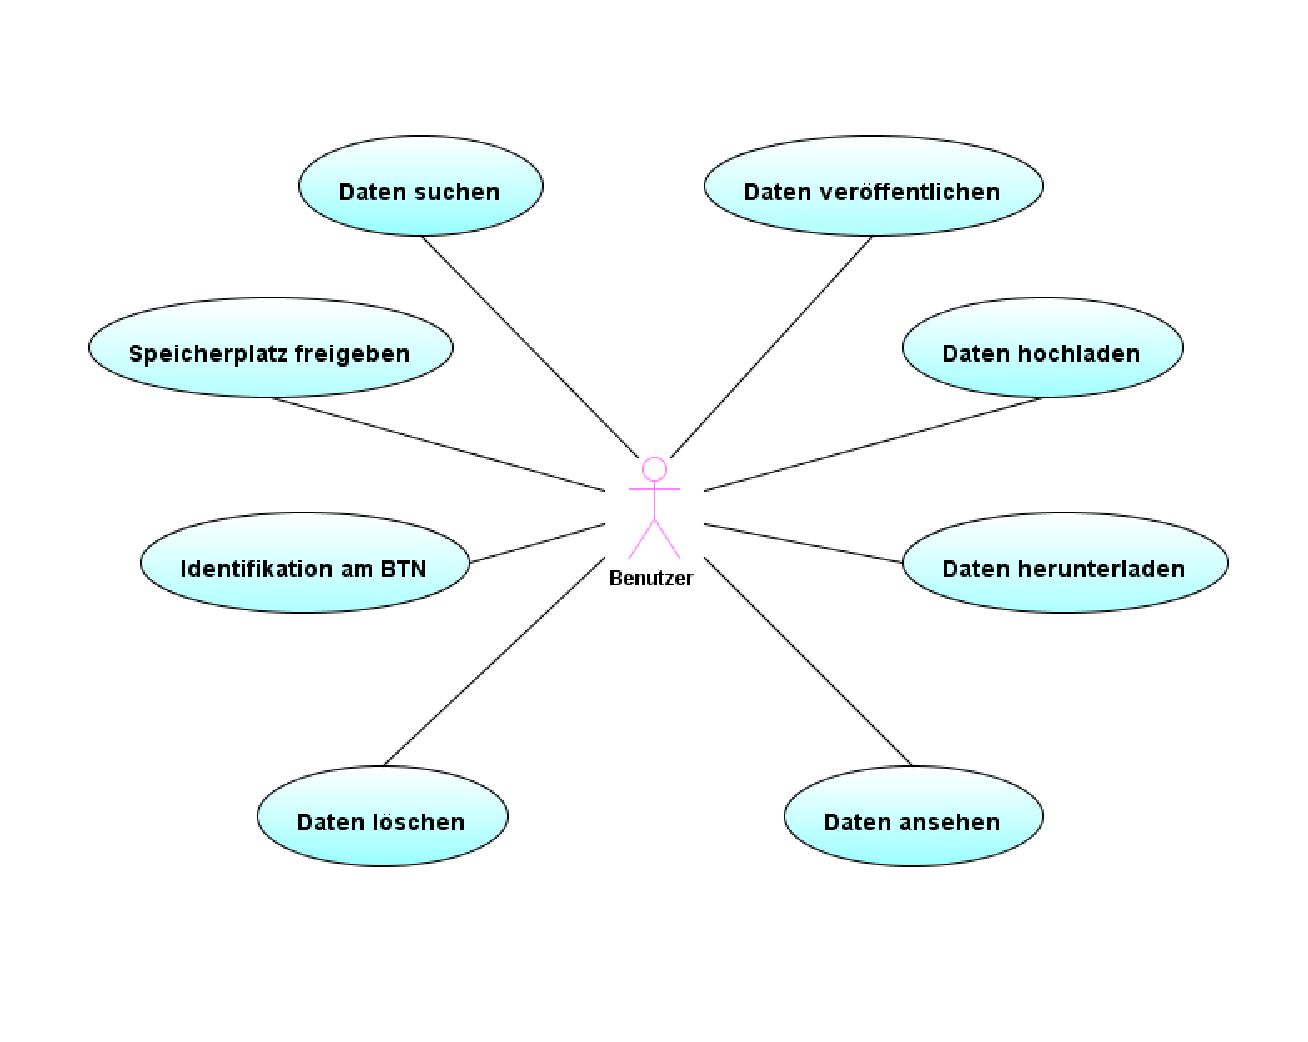
\includegraphics[scale=0.7]{Produktuebersicht.pdf}
		\caption{Übersicht über die Anwendungsfälle aus der Benutzersicht (s. auch Kapitel \ref{sec:usecaseuser}).}
	\end{figure}

	\begin{figure}[hpt]
		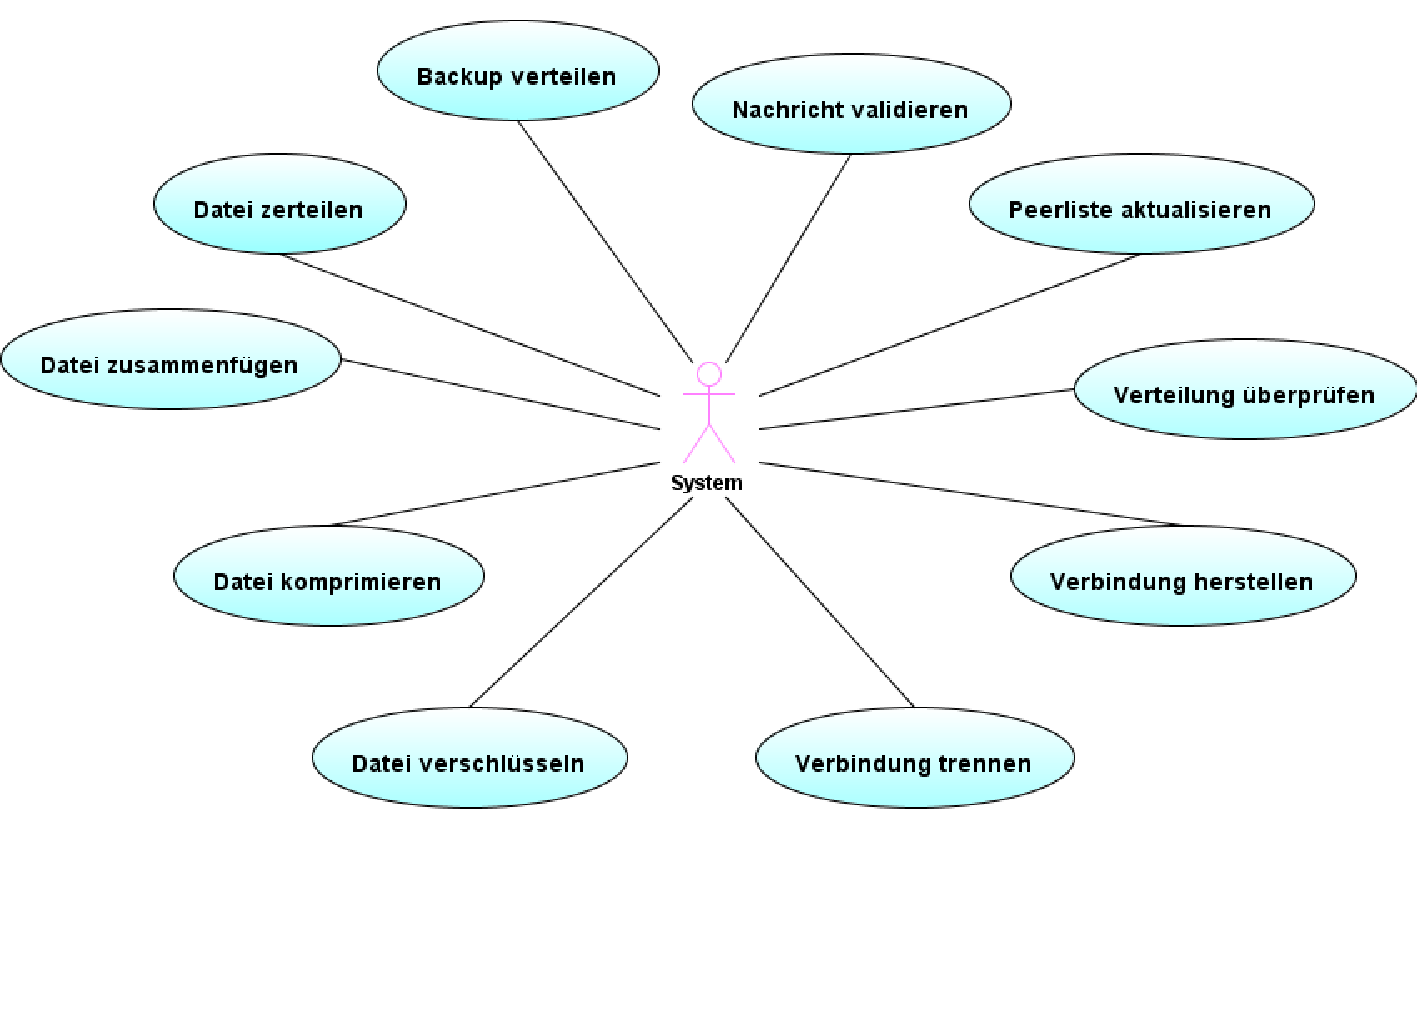
\includegraphics[scale=0.7]{SystemUseCases.pdf}
		\caption{Übersicht über die Anwendungsfälle aus der Systemsicht (s. auch Kapitel \ref{sec:usecasesystem}).}
	\end{figure}

\end{center}

   \clearpage
   \section{Akteure}
 Die nachfolgenden Anwendungsfälle beziehen sich auf den folgenden Akteur:

{\small
\begin{center}
   \begin{tabular}{|l|l|l|}
   \hline
		Akteur		& Beschreibung & Zugehörige Anwendungsszenarios \\
   \hline
		Benutzer	& \begin{minipage}{3.5cm}
					\vspace{0.1cm}
                       Empfängt Backup-Dateiteile, kann Dateien veröffentlichen, 
                       verschickt eine Liste von Dateien, kann Dateien löschen und suchen und lädt Dateien hoch.
                 \end{minipage}
                 \vspace{0.1cm}
               & \begin{minipage}{10cm}
					\vspace{0.1cm}
					\begin{itemize}
						\item Eine eigene, lokale Datei veröffentlichen
						\item Alle veröffentlichten \gls{daten} eines \gls{peer}s anzeigen
						\item Eine Backup-Datei verteilen
						\item Eine veröffentlichte Datei eines \gls{peer}s herunterladen
						\item Speicherplatz für andere freigeben
						\item Identifikation mit Benutzername und Passwort
						\item Eine eigene Backup-Datei aus dem \gls{btn} löschen
						\item Eine veröffentlichte Datei anhand von Stichwörtern suchen
					\end{itemize}
                    \vspace{0.1cm}
                    \end{minipage}\\[0.1cm]
	\hline
		System		& \begin{minipage}{3.5cm}
					\vspace{0.1cm}
						Führt die Aktionen des Benutzers auf unterster Ebene aus, und verwaltet Nachrichten von anderen \gls{peer}s und verarbeitet \gls{daten}.
                 \end{minipage}
                 \vspace{0.1cm}
               & \begin{minipage}{10cm}
					\vspace{0.1cm}
					\begin{itemize}
						\item Verbindung herstellen
						\item Verbindung trennen
						\item Nachricht validieren
						\item \gls{peerliste} aktualisieren
						\item Verteilung überprüfen
						\item Daten verschlüsseln
						\item Daten entschlüsseln
						\item Daten komprimieren
						\item Daten dekomprimieren
						\item Daten teilen
						\item Daten zusammenfügen
						\item \gls{backup}-Daten verteilen
					\end{itemize}
                    \vspace{0.1cm}
                    \end{minipage}\\[0.1cm]
	\hline
	\end{tabular}

\end{center}}

   \clearpage
   \section{Produktfunktionen}

\subsection{Anwendungsfälle aus Benutzersicht}
\label{sec:usecaseuser}

Nachfolgend werden die folgenden Anwendungsfälle detailliert beschrieben: 
\begin{itemize}
	\item Eine eigene, lokale Datei veröffentlichen (Alternativ: mehrere Dateien)
	\item Alle veröffentlichten Daten eines \gls{peer}s anzeigen (Alternativ: alle Peers)
	\item Eine Backup-Datei verteilen (Alternativ: mehrere Backup-Dateien)
	\item Eine veröffentlichte Datei eines \gls{peer}s herunterladen (Alternativ: Backup mit Passwort)
	\item Speicherplatz für andere freigeben
	\item Identifikation mit Benutzername und Passwort
	\item Eine eigene Backup-Datei aus dem \gls{btn} löschen
	\item Eine veröffentlichte Datei anhand von Stichwörtern suchen
\end{itemize}

\subsubsection{Veröffentlichen von lokalen Dateien}
\begin{center}
	\begin{tabular}{|l|p{10cm}|}
		\hline
		Use Case Nummer & V-\useusercounter \\
		\hline
		Use Case Name & Eigene, lokale Datei veröffentlichen \\
		\hline
		Initiierender Akteur & Benutzer \\
		\hline
		Weitere Akteure &  - \\
		\hline
		Kurzbeschreibung & Der Benutzer wählt eine eigene, lokale Datei aus und markiert sie als „ver\-öffentlicht“.\\
		\hline
		Vorbedingung & Die \gls{bta} ist mit dem \gls{btn} verbunden. \\
		\hline
		Nachbedingung & Die Datei wurde veröffentlicht und kann von allen \gls{peer}s angesehen werden. \\
		\hline
		Funktionalität des Use Cases &
		Ablauf:
		\begin{enumerate}
			\item Der Benutzer wählt die eigene, lokale Datei aus
			\item Der Benutzer markiert die Datei als „veröffentlicht“
		\end{enumerate}\\
		\hline
		Alternativen &
		\begin{description}
			\item zu 1) Der Benutzer wählt mehrere Dateien/Ordner aus
			\item zu 2) Abbruch der Auswahl
		\end{description}\\
		\hline
		Ausnahmen & - \\
		\hline
		Benutzte Use Cases & - \\
		\hline
	\end{tabular}
\end{center}

\newpage
 
\subsubsection{Alle veröffentlichten Daten eines Peers anzeigen}
\firstPartUsecaseTable{V-\useusercounter}
{Alle Veröffentlichten Daten eines \gls{peer}s anzeigen}
{Benutzer}
{-}
{Der Benutzer lässt sich alle veröffentlichten Daten eines \gls{peer}s anzeigen}
{Die \gls{bta} ist mit dem \gls{btn} verbunden.}
{Die \gls{bta} zeigt alle Daten eines ausgewählten \gls{peer}s an.}
{Ablauf:\begin{enumerate}\item Der Benutzer wählt einen \gls{peer} aus der aktuellen \gls{peerliste} aus.\item Der Benutzer wählt „Alle veröffentlichten Daten anzeigen“ aus.\item Die \gls{bta} zeigt alle Daten des ausgewählten \gls{peer}s an.\end{enumerate}}
{\begin{description}
	\item zu 1) Der Benutzer wählt mehrere Dateien/Ordner aus.
	\item zu 2) Abbruch der Auswahl.
\end{description}}
Ausnahmen & -\\
\hline
 Benutzte Use Cases & -\\
\hline
\end{tabular}
\end{center}

\newpage

\subsubsection{Eine Backup-Datei verteilen}
\firstPartUsecaseTable{V-\useusercounter}
{Eine Backup-Datei verteilen}
{Benutzer}
{-}
{Der Benutzer wählt eine eigene, lokale Datei aus und markiert sie als „gesichert“.}
{Die \gls{bta} ist mit dem \gls{btn} verbunden.}
{Die Datei wurde gesichert und kann nur von dem Benutzer angesehen werden.}
{Ablauf:\begin{enumerate}\item Der Benutzer wählt die eigene, lokale Datei aus.
\item Der Benutzer markiert die Datei als „gesichert“.\end{enumerate}}
{\begin{description}
	\item zu 1) Der Benutzer wählt mehrere Dateien/Ordner aus.
	\item zu 2) Abbruch der Auswahl.
\end{description}}
Ausnahmen & -\\
\hline
 Benutzte Use Cases & -\\
\hline
\end{tabular}
\end{center}

\newpage

\subsubsection{Eine veröffentlichte Datei herunterladen}
\firstPartUsecaseTable{V-\useusercounter}
{Eine veröffentlichte Datei herunterladen}
{Benutzer}
{-}
{Der Benutzer lädt eine veröffentlichte Datei eines Peers herunter.}
{Die \gls{bta} ist mit dem \gls{btn} verbunden.
Die Liste der öffentlichen Dateien eines \gls{peer}s wird angezeigt.}
{Die \gls{bta} zeigt die heruntergeladene Datei an.}
{Ablauf:\begin{enumerate} \item Der Benutzer wählt eine veröffentlichte Datei eines \gls{peer}s aus der Liste.
\item Der Benutzer lädt diese Datei herunter.\end{enumerate}}
{\begin{description} \item zu 1) Der Benutzer lädt eine von ihm gesicherte Datei herunter, nachdem das richtige  Passwort eingegeben wurde.\end{description}}
Ausnahmen & -\\
\hline
 Benutzte Use Cases & -\\
\hline
\end{tabular}
\end{center}

\newpage

\subsubsection{Speicherplatz für andere freigeben}
\firstPartUsecaseTable{V-\useusercounter}
{Speicherplatz für andere freigeben}
{Benutzer}
{-}
{Der Benutzer wählt einen eigenen, lokalen Ordner und stellt die maximale Größe ein.}
{}
{Ein eigener Ordner ist für die empfangenen Backup-Dateien anderer mit einer maximalen Größe bereit.}
{Ablauf:\begin{enumerate}\item Der Benutzer wählt den eigenen, lokalen Ordner aus.
\item Der Benutzer legt eine maximale Größe fest.\end{enumerate}}
{\begin{description}
	\item zu 2) Abbruch der Auswahl.
\end{description}}
Ausnahmen & -\\
\hline
 Benutzte Use Cases & -\\
\hline
\end{tabular}
\end{center}

\newpage

\subsubsection{Identifikation mit Benutzername und Passwort}
\firstPartUsecaseTable{V-\useusercounter}
{Identifikation mit Benutzername und Passwort}
{Benutzer}
{-}
{Der Benutzer identifiziert sich mit einem Benutzernamen und Passwort.}
{Die \gls{bta} ist mit dem \gls{btn} verbunden.}
{Der Benutzer ist identifiziert.}
{Ablauf: \begin{enumerate} \item Der Benutzer gibt Benutzernamen und Passwort ein.\end{enumerate}}
{\begin{description} \item zu 1) Es erfolgt keine Eingabe seitens des Benutzers.\end{description}}
Ausnahmen & -\\
\hline
 Benutzte Use Cases & -\\
\hline
\end{tabular}
\end{center}

\newpage

\subsubsection{Backup-Datei löschen}
\firstPartUsecaseTable{V-\useusercounter}
{Eigene Backup-Datei löschen}
{Benutzer}
{-}
{Der Benutzer löscht eine seiner Backup-Dateien aus dem \gls{btn}.}
{Die \gls{bta} ist mit dem \gls{btn} verbunden.}
{Die eigene Backup-Datei wurde aus dem \gls{btn} gelöscht.}
{Ablauf: \begin{enumerate} \item Der Benutzer lässt sich die Liste seiner Backup-Dateien anzeigen.
\item Der Benutzer markiert eine Datei aus der Liste. \item Der Benutzer klickt auf „Backup-Datei löschen“.\end{enumerate}}
{\begin{description} \item zu 2) Der Benutzer bricht ab.\end{description}}
Ausnahmen & -\\
\hline
 Benutzte Use Cases & -\\
\hline
\end{tabular}
\end{center}

\newpage

\subsubsection{Veröffentlichte Dateien suchen}
\firstPartUsecaseTable{V-\useusercounter}
{Veröffentlichte Dateien anhand von Stichwörtern suchen}
{Benutzer}
{-}
{Der Benutzer gibt Stichwörter ein und sucht damit nach veröffentlichten Dateien.}
{Die \gls{bta} ist mit dem \gls{btn} verbunden.}
{Die Liste der veröffentlichten Dateien, die zu den Stichwörtern passen, wird angezeigt.}
{Ablauf: \begin{enumerate} \item Der Benutzer gibt Stichwörter ein.
\item Die \gls{bta} zeigt alle veröffentlichten Daten mit den eingegebenen Stichwörtern an.\end{enumerate}}
{-}
Ausnahmen & -\\
\hline
 Benutzte Use Cases & -\\
\hline
\end{tabular}
\end{center}

\newpage

%-------------------------------------------------------------------------------------
%-------------------------------------------------------------------------------------
%-------------------------------------------------------------------------------------

\subsection{Anwendungsfälle aus Systemsicht}
\label{sec:usecasesystem}

Nachfolgend werden die folgenden Anwendungsfälle detailliert beschrieben: 
\begin{itemize}
	\item Verbindung herstellen
	\item Verbindung trennen
	\item Nachricht validieren
	\item \gls{peerliste} aktualisieren
	\item Verteilung überprüfen
	\item Daten verschlüsseln
	\item Daten entschlüsseln
	\item Daten komprimieren
	\item Daten dekomprimieren
	\item Daten teilen
	\item Daten zusammenfügen
	\item \gls{backup}-Daten verteilen
\end{itemize}

\subsubsection{Verbindung herstellen}
\firstPartUsecaseTable{S-\usesystemcounter}
{Eine Verbindung mit dem \gls{btn} herstellen}
{System}
{-}
{Das System stellt eine Verbindung zum \gls{btn} her.}
{Es besteht keine Verbindung zum \gls{btn}. Es ist zu mindestens die Adresse von einem \gls{peer} im \gls{btn} bekannt.}
{Es besteht eine Verbindung zum \gls{btn}.}
{Ablauf:
	\begin{enumerate}
		\item Das System verbindet sich mit dem bekannten \gls{peer}.
	\end{enumerate}}
{-}
Ausnahmen 	& Es konnte keine Verbindung hergestellt werden.\\
\hline
 Benutzte Use Cases & -\\
\hline
\end{tabular}
\end{center}

\newpage

\subsubsection{Verbindung trennen}
\firstPartUsecaseTable{S-\usesystemcounter}
{Die Verbindung mit dem \gls{btn} trennen}
{System}
{-}
{Das System trennt die Verbindung zum \gls{btn}.}
{Es besteht eine Verbindung zum \gls{btn}.}
{Es besteht keine Verbindung zum \gls{btn}.}
{Ablauf:
	\begin{enumerate}
		\item Das System sendet, empfängt und antwortet auf keine Nachrichten mehr.
	\end{enumerate}}
{-}
Ausnahmen 	& -\\
\hline
 Benutzte Use Cases & -\\
\hline
\end{tabular}
\end{center}

\newpage

\subsubsection{Nachricht validieren}
\firstPartUsecaseTable{S-\usesystemcounter}
{Eine eingehende Nachricht validieren}
{System}
{-}
{Das System prüft, ob eine eingehende Nachricht im korrekten Format vorliegt.}
{Das System kennt eine Spezifikation, anhand der es die Korrektheit einer Nachricht nachweisen kann.}
{Die Nachricht wurde als korrekt oder nicht korrekt identifiziert.}
{Ablauf:
	\begin{enumerate}
		\item Das System prüft, ob die eingehende \gls{xml}-Nachricht einem vorgegebenen \gls{xml}-Schema entspricht.
		\item Die Nachricht wird als korrekt identifiziert.
	\end{enumerate}}
{\begin{description}
		\item zu 2) die Nachricht wurde als nicht korrekt identifiziert.
	\end{description}}
Ausnahmen 	& -\\
\hline
 Benutzte Use Cases & -\\
\hline
\end{tabular}
\end{center}

\newpage

\subsubsection{Peerliste aktualisieren}
\label{usecase:peerliste}
\firstPartUsecaseTable{S-\usesystemcounter}
{Peerliste aktualisieren}
{System}
{-}
{Das System prüft, welche \gls{node}s in der \gls{peerliste} online sind und welche offline sind.}
{Es besteht eine Verbindung zum \gls{btn}}
{Das System hält eine aktuelle \gls{peerliste}.}
{Ablauf:
	\begin{enumerate}
		\item Jede Stunde verschickt das System seine \gls{peerliste} an alle \gls{peer}s.
		\item Das System kriegt \gls{peerliste}n von jedem \gls{peer} zurück und setzt das Online-Flag dieses \gls{peer}s auf \texttt{true}.
		\item Das System fügt die fremden Informationen in seine \gls{peerliste} ein.
	\end{enumerate}}
{\begin{description}
		\item zu 2) das System kriegt von einem Knoten keine \gls{peerliste} und setzt das Online-Flag des \gls{peer}s in der \gls{peerliste} auf \texttt{false}. 
	\end{description}}
Ausnahmen 	& -\\
\hline
 Benutzte Use Cases & -\\
\hline
\end{tabular}
\end{center}

\newpage

\subsubsection{Verteilung überprüfen}
\firstPartUsecaseTable{S-\usesystemcounter}
{Die Verteilung von Dateiteilen überprüfen}
{System}
{-}
{Das System prüft, ob die Dateiteile ausreichend im Netz verteilt sind.}
{Das System hat Informationen über die Dateiteile und eine aktuelle \gls{peerliste}. Anforderungen an die Anzahl der Verteilung der Dateiteile.}
{Die Verteilung wurde als ausreichend oder nicht ausreichend gekennzeichnet.}
{Ablauf:
	\begin{enumerate}
		\item Das System schickt an alle \gls{peer}s eine Anfrage, ob sie den Dateiteil x haben.
		\item Das System überprüft, ob die Anzahl der Dateiteile x im System den Anforderungen genügt.
		\item Das System bewertet die Verteilung als ausreichend.
	\end{enumerate}}
{\begin{description}
		\item zu 3) das System bewertet die Verteilung als nicht ausreichend.
	\end{description}}
Ausnahmen 	& -\\
\hline
 Benutzte Use Cases & -\\
\hline
\end{tabular}
\end{center}

\newpage

\subsubsection{Daten verschlüsseln}
\firstPartUsecaseTable{S-\usesystemcounter}
{\gls{daten} mit einem Passwort verschlüsseln}
{System}
{-}
{Das System verschlüsselt die \gls{daten} mit einem Passwort}
{\gls{daten}, die verschlüsselt werden soll. Das System besitzt Zugriffsrechte für die \gls{daten}. Es ist genügend Speicherplatz vorhanden.}
{Die \gls{daten} sind verschlüsselt.}
{Ablauf:
	\begin{enumerate}
		\item Das System liest die \gls{daten} ein.
		\item Das System verschlüsselt die \gls{daten} mit Hilfe eines Verschlüsselungsalgorithmus.
		\item Das System legt die verschlüsselten \gls{daten} ab.
	\end{enumerate}}
{-}
Ausnahmen & Es ist nicht genügend Speicherplatz vorhanden.\\
\hline
 Benutzte Use Cases & -\\
\hline
\end{tabular}
\end{center}

\newpage

\subsubsection{Daten entschlüsseln}
\firstPartUsecaseTable{S-\usesystemcounter}
{\gls{daten} mit einem Passwort entschlüsseln}
{System}
{-}
{Das System entschlüsselt die \gls{daten} mit einem Passwort.}
{\gls{daten}, die entschlüsselt werden soll und verschlüsselt sind. Das System besitzt Zugriffsrechte für die \gls{daten}. Es ist genügend Speicherplatz vorhanden. Ein Passwort ist vorhanden.}
{Die \gls{daten} sind entschlüsselt.}
{Ablauf:
	\begin{enumerate}
		\item Das System liest die \gls{daten} ein.
		\item Das System entschlüsselt die \gls{daten} mit Hilfe eines Verschlüsselungsalgorithmus und dem Passwort.
		\item Das System legt die entschlüsselten \gls{daten} ab.
	\end{enumerate}}
{\begin{description}
		\item zu 3) die \gls{daten} wurden nicht erfolgreich entschlüsselt, weil das Passwort falsch war.
	\end{description}}
Ausnahmen & Es ist nicht genügend Speicherplatz vorhanden.\\
\hline
 Benutzte Use Cases & -\\
\hline
\end{tabular}
\end{center}

\newpage

\subsubsection{Daten komprimieren}
\firstPartUsecaseTable{S-\usesystemcounter}
{\gls{daten} komprimieren}
{System}
{-}
{Das System komprimiert die \gls{daten}.}
{\gls{daten}, die komprimiert werden soll. Das System besitzt Zugriffsrechte für die \gls{daten}. Es ist genügend Speicherplatz vorhanden.}
{Die \gls{daten} sind komprimiert.}
{Ablauf:
	\begin{enumerate}
		\item Das System liest die \gls{daten} ein.
		\item Das System komprimiert die \gls{daten} mit Hilfe eines Komprimierungsalgorithmuses.
		\item Das System legt die komprimierten \gls{daten} ab.
	\end{enumerate}}
{-}
Ausnahmen & Es ist nicht genügend Speicherplatz vorhanden.\\
\hline
 Benutzte Use Cases & -\\
\hline
\end{tabular}
\end{center}

\newpage

\subsubsection{Daten dekomprimieren}
\firstPartUsecaseTable{S-\usesystemcounter}
{\gls{daten} dekomprimieren}
{System}
{-}
{Das System dekomprimiert die \gls{daten}.}
{\gls{daten}, die dekomprimiert sind. Das System besitzt Zugriffsrechte für die \gls{daten}. Es ist genügend Speicherplatz vorhanden.}
{Die \gls{daten} sind dekomprimiert.}
{Ablauf:
	\begin{enumerate}
		\item Das System liest die \gls{daten} ein.
		\item Das System dekomprimiert die \gls{daten}.
		\item Das System legt die dekomprimierten \gls{daten} ab.
	\end{enumerate}}
{-}
Ausnahmen & Es ist nicht genügend Speicherplatz vorhanden.\\
\hline
 Benutzte Use Cases & -\\
\hline
\end{tabular}
\end{center}

\newpage

\subsubsection{Daten teilen}
\firstPartUsecaseTable{S-\usesystemcounter}
{\gls{daten} teilen in mehrere kleinere Dateiteile}
{System}
{-}
{Das System teilt die \gls{daten} in mehrere kleinere Dateiteile.}
{\gls{daten}, die geteilt werden sollen. Das System besitzt Zugriffsrechte für die \gls{daten}. Es ist genügend Speicherplatz vorhanden.}
{Die \gls{daten} sind geteilt in mehrere kleinere Dateiteile.}
{Ablauf:
	\begin{enumerate}
		\item Das System komprimiert die \gls{daten} und teilt dabei die \gls{daten} in mehrere kleinere Dateiteile.
		\item Das System legt die Dateiteile ab.
	\end{enumerate}}
{-}
Ausnahmen & Es ist nicht genügend Speicherplatz vorhanden.\\
\hline
 Benutzte Use Cases & -\\
\hline
\end{tabular}
\end{center}

\newpage

\subsubsection{Daten zusammenfügen}
\firstPartUsecaseTable{S-\usesystemcounter}
{Dateiteile zusammenfügen zu den originalen \gls{daten}}
{System}
{-}
{Das System fügt die Dateiteile zu den originalen \gls{daten} zusammen.}
{Dateiteile, die zusammengefügt werden sollen und alle Dateiteile zu den originalen \gls{daten}. Das System besitzt Zugriffsrechte für die Dateiteile. Es ist genügend Speicherplatz vorhanden.}
{Die originalen \gls{daten} stehen wieder zur Verfügung.}
{Ablauf:
	\begin{enumerate}
		\item Das System dekomprimiert die \gls{daten} aus den Dateiteilen.
		\item Das System legt die \gls{daten} ab.
	\end{enumerate}}
{-}
Ausnahmen & Es ist nicht genügend Speicherplatz vorhanden.\\
\hline
 Benutzte Use Cases & -\\
\hline
\end{tabular}
\end{center}

\newpage

\subsubsection{Backup-Daten verteilen}
\firstPartUsecaseTable{S-\usesystemcounter}
{\gls{backup}-\gls{daten} verteilen}
{System}
{\gls{peer}}
{Das System verteilt eine \gls{backup}-Datei redundant an mehrere \gls{peer}s.}
{Es besteht eine Verbindung zum \gls{btn}, die zu verteilenden \gls{daten} sind komprimiert, verschlüsselt und aufgeteilt worden und die zugehörigen Meta-\gls{daten} sind verschlüsselt worden.}
{Die \gls{backup}-\gls{daten} wurden vollständig gemäß der \gls{redqua} verteilt.}
{Ablauf:
	\begin{enumerate}
		\item Das System öffnet einen \gls{tcp}-\gls{port}.
		\item Das System sendet solange sukzessiv Speicher-Anfragen (\ref{sec:speicheranfrage}) (mit dem geöffneten \gls{tcp}-\gls{port}) pro \gls{btfp} von den zu verteilenden \gls{backup}-\gls{daten}  gemäß der \gls{redqua} an verschiedene \gls{peer}s aus der eigenen \gls{peerliste}, bis alle \gls{btfp} erfolgreich versandt wurden.
		\item Jeder \gls{peer}, der einen \gls{btfp} speichern kann, lädt einen solchen über den \gls{tcp}-\gls{port} herunter.
		\item Bei kompletter, erfolgreicher Übertragung schließt das System den geöffneten \gls{tcp}-\gls{port}.
	\end{enumerate}}
{-}
Ausnahmen & zu 2.) Das System kann keine Verbindung zum \gls{peer} herstellen: Das Online-Flag (\ref{usecase:peerliste}) wird auf false gesetzt und die Speicher-Anfrage wird an einen anderer \gls{peer} gesendet.\\
	& zu 2.) Das System konnte nicht alle \gls{btfp} gemäß der \gls{redqua} versenden: Das System benachrichtigt Benutzer.\\
\hline
 Benutzte Use Cases & -\\
\hline
\end{tabular}
\end{center}

   \clearpage
   \section{Produktdaten}
Es werden nachfolgend alle Daten und Datenstrukturen angegeben, die die \gls{bta} speichert und benutzt:

\subsection{Peerliste und Nodes}
Die \gls{bta} hält eine Liste (die sogenannte \gls{peerliste}) mit allen \gls{node}s im \gls{btn}, wobei jede \gls{node} mit folgenden Informationen gespeichert wird:
\begin{itemize}
	\item \gls{ip}-Adresse
	\item \gls{udp}-\gls{port}
	\item Zeitstempel der letzten Aktivität des \gls{node}s
	\item Gesamter Speicherplatz
	\item Freier Speicherplatz
	\item Online-Flag \ref{usecase:peerliste}
\end{itemize}

{\Large Die empfangenen Dateiteile werden lokal mit einem zusätzlichen Informationsteil abgelegt, der wie folgt aussieht}:

\subsection{Veröffentlichte Dateien}
\begin{itemize}
	\item \gls{hash} \"uber die Meta-Daten und die Daten
	\item Meta-Daten:
	\begin{itemize}
		\item Titel
		\item Schl\"usselw\"orter
		\item Benutzername des Autors
		\item Teil x von y
		\item Datum und Uhrzeit der letzten \"Anderung
		\item Gesamt-\gls{hash}
	\end{itemize}
\end{itemize}

\newpage

\subsection{Sicherungsdateien}
\begin{itemize}
	\item Benutzername des Autors
	\item Benutzername des Autors (verschl\"usselt)
	\item \gls{hash} \"uber die verschl\"usselten Meta-Daten und die verschl\"usselten Daten
	\item Meta-Daten (verschl\"usselt):
		\begin{itemize}
			\item Titel
			\item Teil x von y
			\item Datum und Uhrzeit der letzten \"Anderung
			\item Gesamt-\gls{hash}
			\item \gls{Part-Passwort}
		\end{itemize}
\end{itemize}

   \clearpage
   \section{Produktleistungen} 

\begin{description}
  \item {\bfseries Ausfallsicherheit:} Nach der manuellen Eingabe eines \gls{peer}s versucht die \gls{gbta} unmittelbar den \gls{peer} zu kontaktieren und bei Erfolg die \gls{node}s des \gls{peer}s abzufragen, um bei Ausfall des initialen \gls{peer}s weiterhin am \gls{gbtn} teilnehmen zu können.
  \item {\bfseries Korrekte Dateiübertragung:} Das korrekte Übertragen 
eines Dateiteils wird durch \gls{tcp}/\gls{ip} übernommen. Hierdurch ist eine komplette und korrekte Übertragung eines Dateiteils bereits sichergestellt.
  \item {\bfseries Verschlüsselung:} Eine Sicherungsdatei wird verschlüsselt im \gls{btn} verteilt. So wird erreicht, dass kein Unbefugter Zugriff auf die \gls{daten} hat.
  \item {\bfseries Komprimierung:} Die Dateien und die Zusatzinformationen zu diesen werden komprimiert und danach erst übertragen. Auf diese Weise ist eine möglichst ressourcenschonende Belastung des Netzwerkes gewährleistet.
    \item {\bfseries Aufteilen der Dateien:} Durch das Aufteilen von einer Datei in mehrere kleinere Dateiteile erreicht das Produkt eine höhere Geschwindigkeit bei der Verteilung der Dateien. Da ein \gls{peer} dadurch von mehreren \gls{peer}s gleichzeitig die gleiche Datei aber andere Dateiteile herunterladen kann. Diese Funktion bietet auch eine effizientere Möglichkeit der Verteilung der Sicherungsdateien.
\end{description}

   \clearpage
   \section{Benutzeroberfläche}
 In diesem Kapitel wird die Benutzeroberfläche der \gls{gbta} sowie ein 
 entsprechender Entwurfsvorschlag vorgestellt.

\begin{figure}[ht]
	\begin{center}
	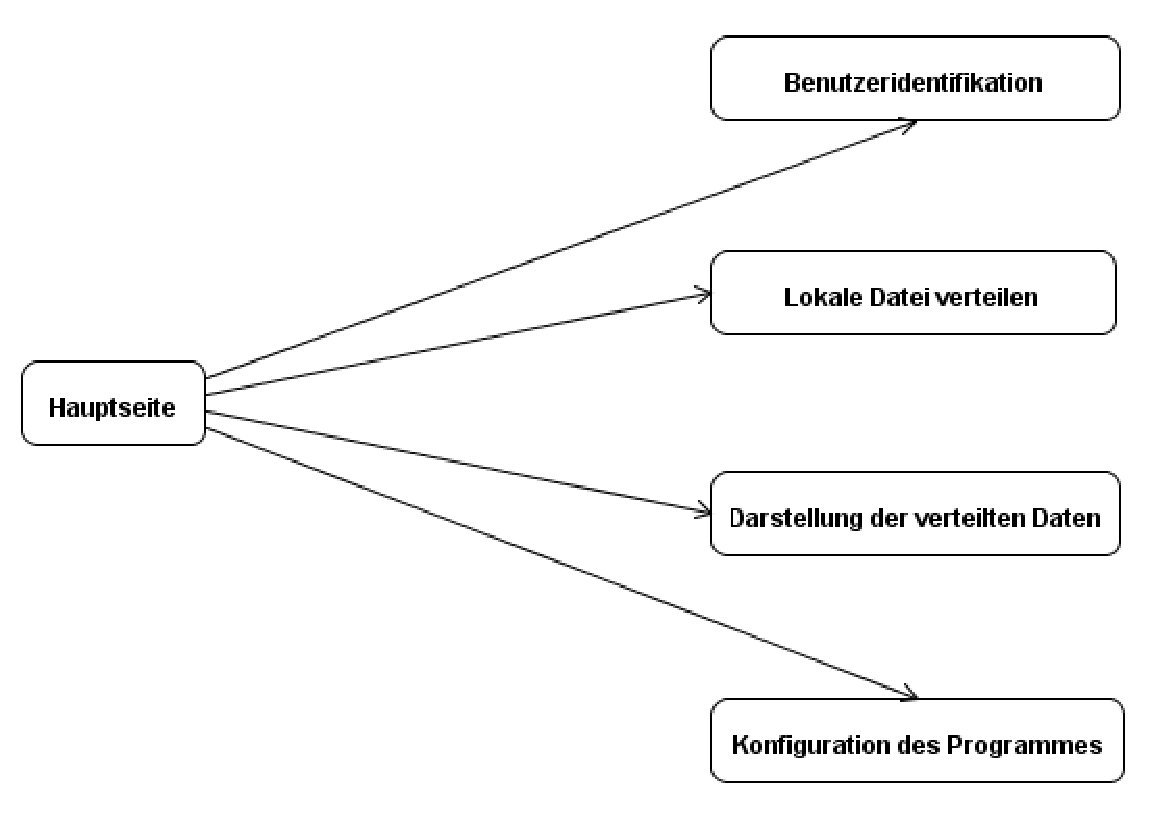
\includegraphics[scale=0.8]{GUIZentral}	
	\end{center}
	\caption{Die Benutzeroberfläche (schematisch).}
\end{figure}

  \subsection{Dialogstruktur}
  Für die Benutzerführung ist die nachfolgende Dialogstruktur vorgesehen, die sich aus 
  den nachfolgenden Komponenten zusammensetzt:
  \begin{enumerate}[1.)]
   \item Einem Dialog zum Anmelden an das System. Eine Abmeldung ist nicht vorgesehen. Eingabe ist die
Benutzerkennung sowie ein Kennwort.

   \item Eine Dialogbox wird verwendet für die Konfiguration von BaseTorrent, d.h. der Eingabe eines Verzeichnisses,
der beim Ablegen von verteilten Dateien und Ordnern verwendet wird. Zudem wird eine maximale Speichergröße
  als auch ein zusätzliches Verzeichnis hinterlegt. Beides wird herangezogen um anderen Benutzern auf dem
  vorliegenden Rechner Speicherkapazität zum Verteilen von Dateien im Netzwerk bereitzustellen.

   \item Die Darstellung von bereits veröffentlichten Dateien und Ordnern sowie, sofern der Benutzer sich gemäß 1.)
  angemeldet hat, auch der benutzerbezogenen Daten.  Diese können in zwei separaten, wenn auch weitestgehend
identisch aufgebauten Komponenten dargestellt werden.

   \item Eine Dialogbox zeigt den Fortschritt des Speicherns von verteilten Daten (der sogenannte \emph{Download}) an.
   \item Eine weitere Dialogbox zeigt ein Eingabefeld an, um nach Dateien mit einem bestimmten Schlüsselwort zu suchen.
  \end{enumerate}

  \subsection{Bildschirmlayout}
  Um eine intuitive Benutzerführung zu gewährleisten wird ein Layout entsprechend 
  der Programmierrichtlinien für die Gestaltung der Benutzeroberflächen von  
  Desktop-Applikationen angestrebt\footnote{Etwa \emph{Microsoft Inductive User Interface Guidelines, http://msdn.microsoft.com/en-us/library/ms997506.aspx}.}. Dies impliziert insbesondere eine einheitliche
Bezeichnung von Schaltflächen und Menüpunkten. Eine Umsetzung mittels Java Swing wird angestrebt. 

 \subsection{GUI-Entwurfsvorschläge}
  Nachfolgend stellen wir einen  Entwurf der Benutzeroberfläche dar.


   \clearpage
   \section{Protokoll}
% ü ä ß damit jeder editor diese datei als utf8 abspeichern kann

\subsection{Beschreibung}
Das Protokoll von BaseTorrent basiert auf Nachrichtenübermittlung mit \gls{udp} und Datenübermittlung mit \gls{tcp}.\\
Bei Verlust von \gls{udp}-Nachrichten wird nach einer einstellbaren Wartezeit erneut gesendet.\\
Die Suchnachrichten werden gestaffelt versendet, d.h. aus der Liste der \gls{node}s werden der Reihe nach eine gewisse Anzahl an \gls{node}s angeschrieben, um das Netzwerk nicht unnötig zu belasten.

\subsubsection{\texttt{status}-Nachricht}
\label{sec:statusmeldung}
\msgtab{Informiert die bekannten \gls{peer}s aus der eigenen \gls{peerliste}, dass man noch mit dem \gls{btn} verbunden ist.}
{\gls{udp}}
{aktuelle \gls{peerliste}}
{\begin{enumerate}
	\item Prüfe die Liste auf Aktualität 
	\item Sende die eigene aktualisierte \gls{peerliste}
\end{enumerate}}


\subsubsection{\texttt{get}-Nachricht}
\label{proto:get}
\msgtab{\gls{daten}-\gls{btfp}-Anfrage an \gls{peer} X, um Daten von X auf den \gls{bta}-Computer zu kopieren.}
{\gls{udp}}
{\gls{btfp}-\gls{hash}, ein eigener \gls{tcp}-\gls{port}}
{\begin{enumerate} \item Lädt die Daten, wenn sie existieren, über den \gls{tcp}-\gls{port} hoch \end{enumerate}}


\subsubsection{\texttt{store}-Nachricht}
\label{sec:speicheranfrage}
\msgtab{Frage an, wer die eigenen Daten aufnehmen kann.}
{\gls{udp}}
{Part-Hash, Metadaten, \gls{tcp}-\gls{port}, Dateigröße}
{\begin{enumerate}
	\item Prüfe auf Vorhandensein
	\item Prüfe freien Speicherplatz
	\item Wenn beides vorhanden, dann Datei herunterladen
\end{enumerate}}


\subsubsection{\texttt{find}-Nachricht}
\label{sec:dateianfrage}
\msgtab{Anfrage an Peer, ob er Datei x hat.}
{\gls{udp}}
{Liste mit Schlüsselwörtern}
{\begin{enumerate}
	\item Prüfe auf Vorhandensein der Datei.
	\item Wenn Datei vorhanden, dann antwortet mit den Metadaten
\end{enumerate}}


\subsubsection{\texttt{meta}-Nachricht}
\label{sec:metaantwort}
\msgtab{Antwort, ob Peer eine Datei x hat.}
{\gls{udp}}
{Metadaten}
{\begin{enumerate}
	\item Antwortet mit den Metadaten
\end{enumerate}}


\subsubsection{\texttt{listBackups}-Nachricht}
\label{sec:backupanfrage}
\msgtab{Anfrage ob Peer BackUps vom Autor y hat.}
{\gls{udp}}
{Autor}
{\begin{enumerate}
	\item Wenn Datei vorhanden, dann "Meta Antwort"
\end{enumerate}}

\subsubsection{\texttt{deleteBackups}-Nachricht}
\label{sec:backuploeschen}
\msgtab{Löschen von Backups.}
{\gls{udp}}
{\gls{btfp}-\gls{hash}, \gls{Part-Passwort}}
{\begin{enumerate}
	\item Prüfe auf Vorhandensein der Datei.
	\item Prüfe auf Übereinstimmung von Autor und durch \gls{Part-Passwort} entschlüsseltem Autor
	\item Wenn Bedingungen erfüllt, dann Datei löschen
\end{enumerate}}

\subsubsection{\texttt{checkParts}-Nachricht}
\label{sec:redundanzpruefen}
\msgtab{Fragt nach, wie oft ein gewisser Part noch im Netz vorhanden ist.}
{\gls{udp}}
{Liste von Part-Hashes}
{\begin{enumerate}
	\item Prüfe auf Vorhandensein der Datei
	\item Wenn Datei vorhanden, dann "Meta Antwort"
\end{enumerate}}

\newpage

\subsection{Zulässige Nachrichtensequenzen}
Die folgenden Sequenzdiagramme zeigen die zulässigen interessanten Nachrichtensequenzen auf (bei den anderen ist dies trivial):
\begin{figure}[hpt]
	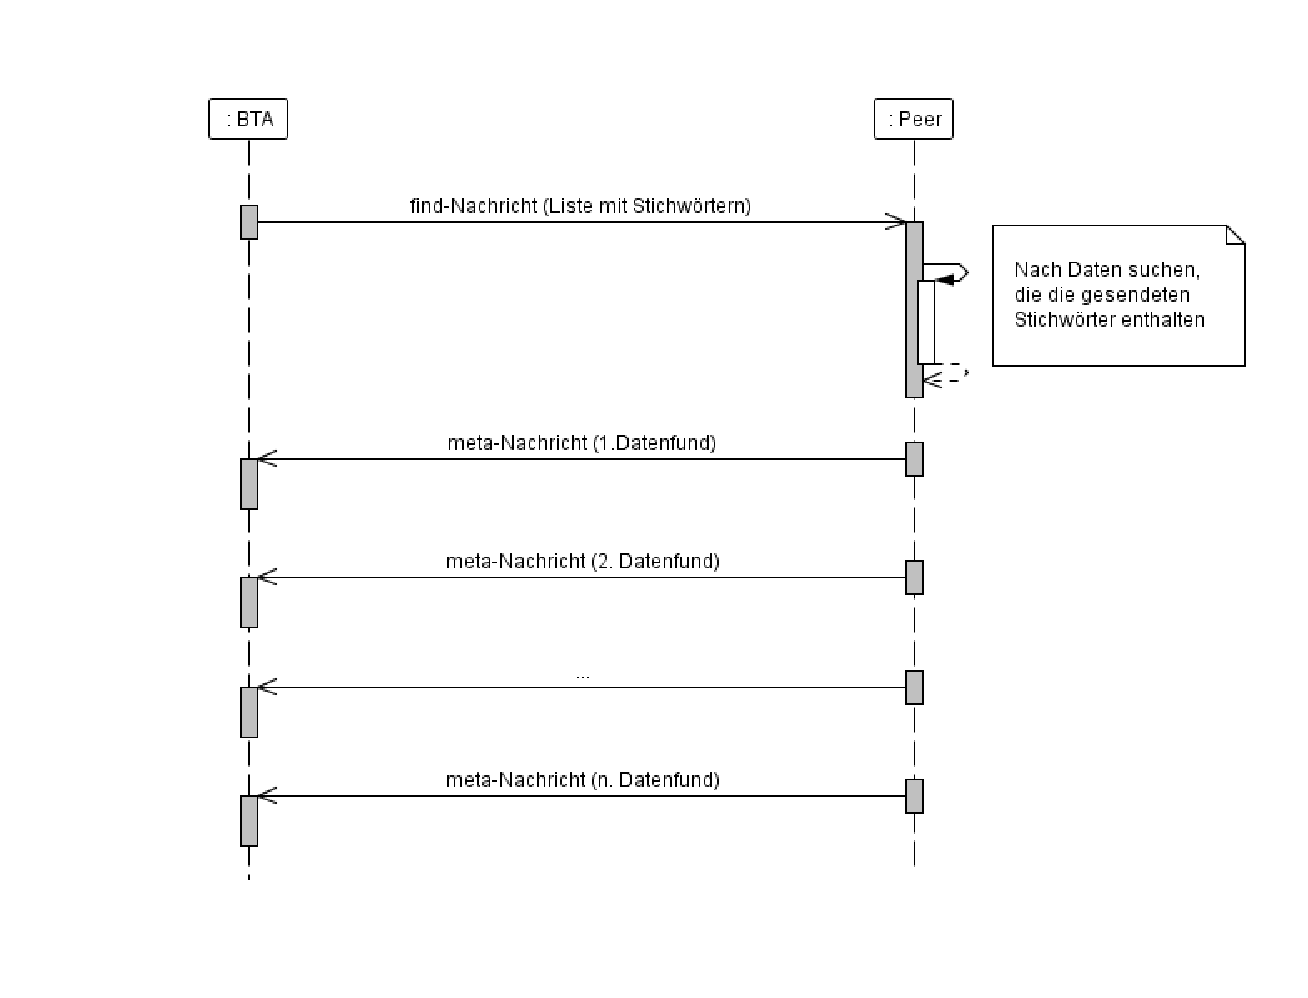
\includegraphics[width=\linewidth]{find.pdf}
	\caption{Beispiel für eine zulässige Suchanfrage}
\end{figure}

\begin{figure}[hpt]
	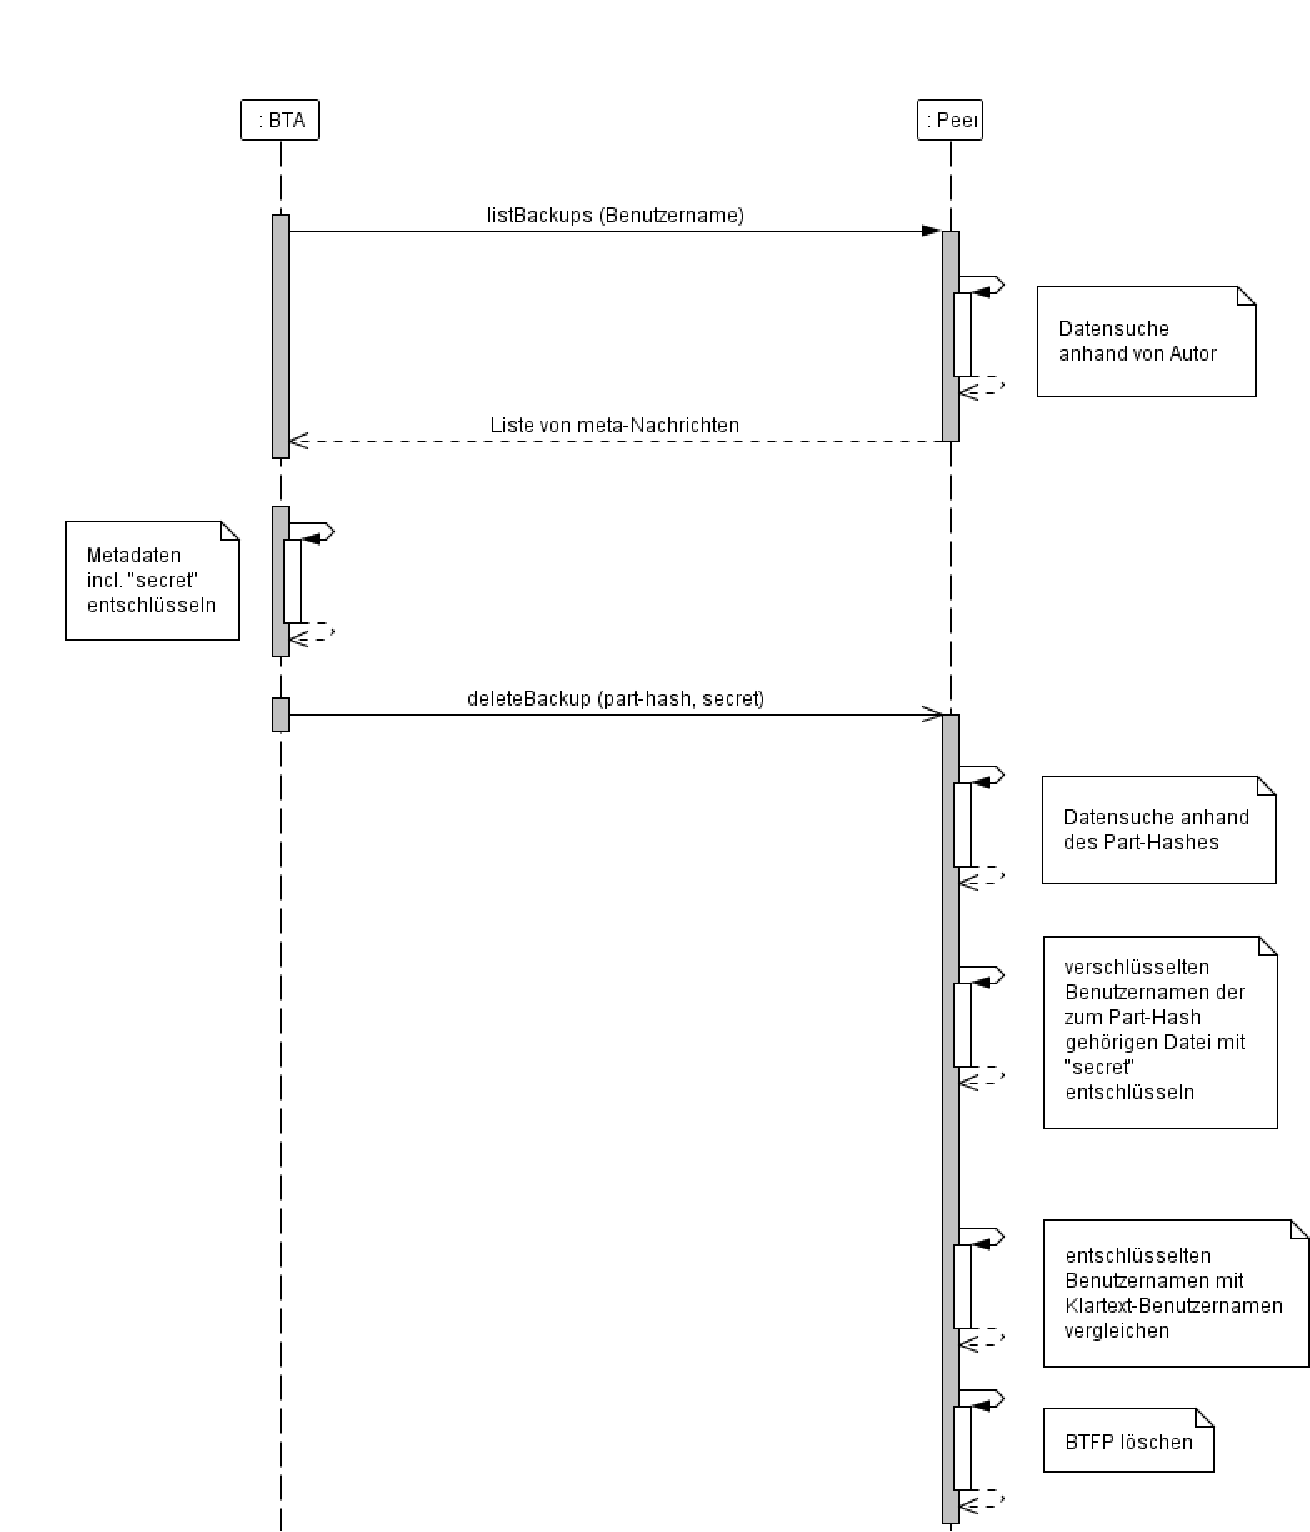
\includegraphics[width=\linewidth]{deleteBackup.pdf}
	\caption{Beispiel für eine zulässige Löschanfrage}
\end{figure}

   \clearpage
   \section{Qualitätsanforderung}

  \vspace{0.5cm}

  \begin{center}
     \begin{tabular}{|l||c|c|c|c|}
\hline
                   & sehr wichtig & wichtig & weniger wichtig & unwichtig \\
\hline
      Robustheit				& x & & &   \\
\hline
      Zuverlässigkeit			& x & & & \\
\hline
      Benutzerfreundlichkeit	& & x & &  \\
\hline
      Effizienz					& & x & & \\
\hline
      Portierbarkeit			& & x & & \\
\hline
      Kompatibilität			& & x & &  \\
\hline
     \end{tabular}
  \end{center}

   \clearpage
   \section{Testszenarien}
Die folgenden Szenarien werden besonders ausgiebig getestet, um optimale Produktqualit\"at zu erreichen:
\subsection{Share-Szenarien}
\begin{itemize}
	\item Benutzer X \underline{ver\"offentlicht} eine Datei z, anschlie\ss{}end holt sich Benutzer Y die Ver\"offentlichungsliste von Benutzer X und kontrolliert, dass die neue Datei z vorhanden ist (\textit{erfolgreiche Ver\"offentlichung}).
	\item Benutzer X \underline{entfernt} eine veröffentlichte Datei z aus seiner Ver\"offentlichungsliste, ruft anschlie\ss{}end seine eigene Ver\"offentlichungsliste ab und kontrolliert, dass die Datei z nicht in der Liste angezeigt wird (\textit{korrekte Share-L\"oschung}).
\end{itemize}

\subsection{Backup-Szenarien}
\begin{itemize}
	\item Der Benutzer \underline{verteilt} eine Backup-Datei, ruft anschlie\ss{}end seine eigenen Backup-Dateien ab und kontrolliert, ob die neue Backup-Dateien (h\"aufig genug) im \gls{btn} vorhanden ist (\textit{erfolgreiche Backup-Verteilung}).
	\item Der Benutzer \underline{l\"oscht} eine Backup-Datei, ruft anschlie\ss{}end seine eigenen Backup-Dateien ab und kontrolliert, dass die gel\"oschte Datei nicht mehr im \gls{btn} vorhanden ist (\textit{erfolgreiche Backup-L\"oschung}).
	\item Der Benutzer ruft seine eigenen Backup-Dateien ab und schl\"agt beim Versuch, eine seiner Backup-Dateien mit einem \underline{falschen Passwort} zu l\"oschen, fehl (\textit{Backup-Sicherheit}).
	\item Benutzer X \underline{verteilt} eine Backup-Datei z (u.a. an Benutzer Y), Benutzer Y trennt sich vom \gls{btn}, Benutzer X l\"oscht lokal die Backup-Datei z, ruft anschlie\ss{}end seine eigenen Backup-Dateien ab und kontrolliert, ob die neue Backup-Datei z weiterhin \underline{vollst\"andig} im \gls{btn} verf\"ugbar ist (\textit{Ausfallsicherheit}).
	\item Der Benutzer verteilt \underline{zwei Backup-Dateien mit demselben Namen}, ruft anschlie\ss{}end seine eigenen Backup-Dateien ab und kontrolliert, ob die beiden neuen Backup-Dateien im \gls{btn} verf\"ugbar sind (\textit{korrekte Backup-Verteilung}).
	\item Der Benutzer \underline{verteilt} eine Backup-Datei z. Benutzer Y ruft die ver\"offentlichten Dateien von Benutzer X ab und kontrolliert, dass die Backup-Datei z von Benutzer X nicht angezeigt wird (\textit{Backup-Sichtbarkeit}).
\end{itemize}

%\subsection{andere Szenarien}
%\begin{itemize}
%	\item 
%\end{itemize}

   \clearpage
   \section{Entwicklungsumgebung}

 \subsection{Software}
  \begin{itemize}
   \item Plattform
     \begin{itemize}
       \item Java, 
       \item Subversion.
     \end{itemize}

    \item Werkzeuge
    \begin{itemize}
     \item Eclipse,
      \item OpenOffice,
      \item Adobe Acrobat Reader,
      \item \LaTeX
    \end{itemize}
  \end{itemize}

 \subsection{Hardware}
  \begin{itemize}
   \item Mindestens vier Personal Computer mit Internetzugang.
  \end{itemize}

 \subsection{Orgware}

   \clearpage
   \appendix
   \section{Anhang}
\label{sec:anhang}
% hier die XML Dateien rein und drauf verweisen ü
\subsection{XML Nachrichten-Schemata}
\label{anhang:xml}
\lstset{tabsize=2, language=XML, numbers=left, basicstyle=\footnotesize, inputencoding=utf8x, extendedchars=\true}
\lstinputlisting{BASETorrent.xsd}

	\clearpage
	\printglossaries
\end{document}
